\documentclass{article}
\usepackage[utf8]{inputenc}

\title{Clarification of Next best underwater view}
\author{mauhing.yip }
\date{October 2020}

\usepackage{natbib}
\usepackage{graphicx}

\begin{document}

\maketitle

\section{Introduction}
I feel that I should have done a better job to clarify something on the NBUV paper that can be easily misunderstood such that we can agree something in the same page. The next best underwater view is quite different from the general next best view in CV/robotic community.

\section{In theory}
In theory based, next best veiw means you have to define your own definition of information. And you have a set of action you can take in next move. you will calculate which one of the action that give you the best information gain. Then, you perform "that" action in the next move. The word "view" is not necessary a camera, it could be sonar, like the paper of Narcis Palomeras. \textbf{Here, different definition of information will define different goal}, it can be the shape of surrounding or texture of object and etc... Therefore, NBV is a broad concept and One need to know definition of information to know what is the \textbf{``best view''} for. 

\section{In general CV/Robotic}
But in general CV/Robotic community (if my experience is good enough), we have a common definition of information. It is the shape of surrounding. To be more specific, it is the number of explored space (if you divide space into small cube). Next best view will explore the most unknown space to obtain more explored space. At the end, this will give you the shape of surrounding, 2D or 3D. It is an explorational NBV algorithm. 

\section{In article of NBUV of Sheinin}
But the article "Next best underwater view" of Sheinin and Schechner, which is my Ph.D topic and starting point article, \textbf{they have very different definition of information. It is the texture of surface and the quality of the texture surface in the entire scene.} This can be addressed in the question like: Given a entire (global) 3D mesh of the scene without any texture, estimate the best pose for light and camera to reduce back-scattering to get the most of texture of the surface. How to calculate the best pose is all based on ocean optic physics. And they assumed you used sonar to get topography (3D mesh). The big drawback for us is the topography (usually is 3D mesh) of the entire scene has to be given, not just locally. \textbf{The NBUV from Sheinin dose not explore outside the given topology (3D mesh/ dense point cloud). It is not an explorational NBV algorithm.} The job of NBUV from Sheinin is to gain texture of entire scene and maximize the quality of the texture with consideration of ocean optic.  We maybe able to overcome this drawback by structure form Motion, it will be discuss later. Some of the figure from the article \cite{sheinin2016next} is shown in \ref{fig:NBUV_txture}, \ref{fig:simulation}, \ref{fig:experiment_1} and \ref{fig:experiment_2}.

(They does not provide any reference of the formulae and the formulae is not correct due the unit. Therefore, I spent A LOT time to correct and back and fort.)

\begin{figure}[h!]
\centering
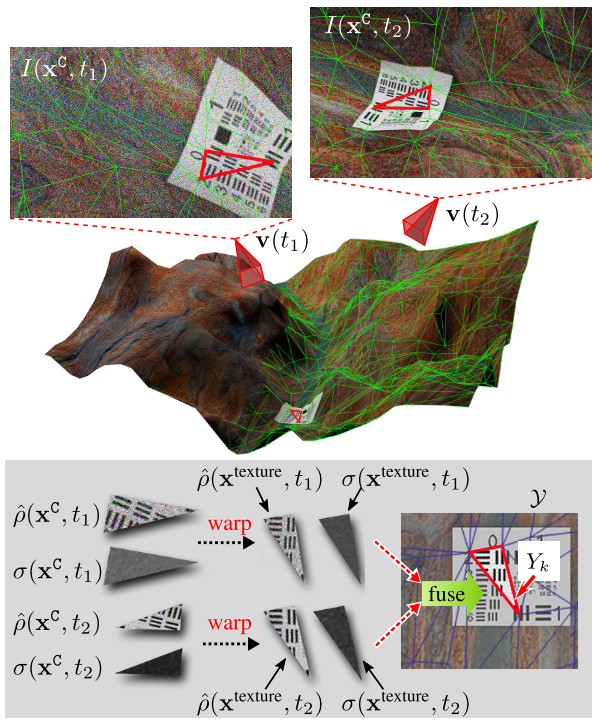
\includegraphics[width=\textwidth]{NBUV_texture_fusion.png}
\caption{\textbf{NBUV texture fusion:} Two pieces of texture from the same surface patch, but different angles. In the article \cite{sheinin2016next}. They how to fused them to obtain a more clear texture. Source: \cite{sheinin2016next}}
\label{fig:NBUV_txture}
\end{figure}

\begin{figure}[h!]
\centering
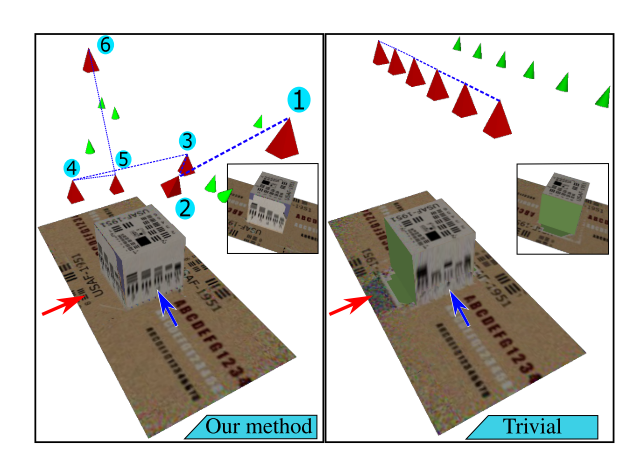
\includegraphics[width=\textwidth]{NBUV_simulation.png}
\caption{\textbf{Simulation:} NBUV compare to fixed camera and light pose.}
\label{fig:simulation}
\end{figure}

\begin{figure}[h!]
\centering
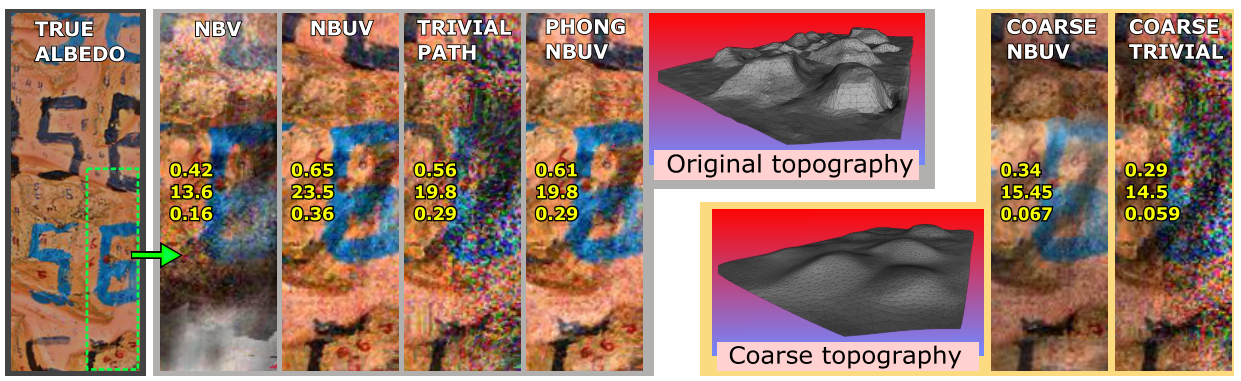
\includegraphics[width=\textwidth]{NBUV_experiment_1.png}
\caption{\textbf{Real world experiment result:} Authors used kinect time of flight camera to obtain the topology in clear medium}
\label{fig:experiment_1}
\end{figure}

\begin{figure}[h!]
\centering
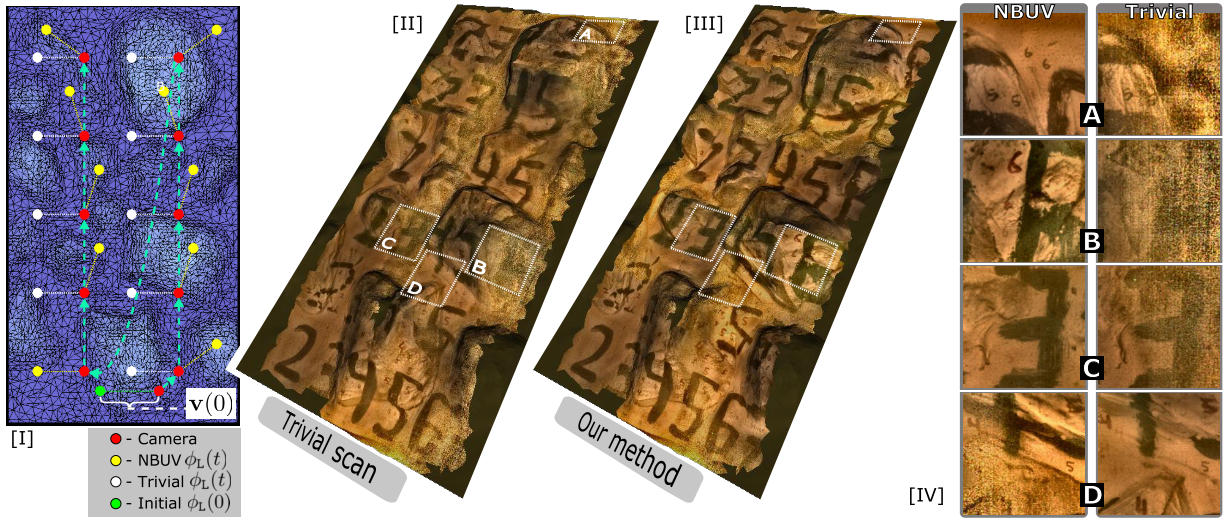
\includegraphics[width=\textwidth]{NBUV_experiment_2.png}
\caption{\textbf{Real world experiment result:} NBUV compare to fixed camera and light pose.}
\label{fig:experiment_2}
\end{figure}



\section{Conclusion}
``I always thought something was fundamentally wrong with the universe'' \citep{adams1995hitchhiker}

\bibliographystyle{plain}
\bibliography{references}
\end{document}
